\section{Maximo cercano}

Este es un filtro tal que cada pixel de la imagen original se edita de la siguiente manera:

\begin{enumerate}
	\item Obtenemos los píxeles de alrededor, que se encuentren a una distancia menor a 3 píxeles.
	\item Se calcula el máximo valor para cada componente entre estos píxeles obtenidos.
	\item Se genera un nuevo píxel con estas 3 valores encontrados.
	\item El píxel final se calcula mediante una combinación lineal entre el píxel original y el píxel que contiene las componentes máximas.
\end{enumerate}

El conjunto de píxeles en donde se busca el máximo valor de cada componente, se lo conoce como kernel y en este caso es de 7x7 píxeles.\\
La combinación lineal entre los píxeles se hace de la siguiente manera:
\begin{center}
$src * (1 - val) + max * (val)$
\end{center}
Donde $src$ es el píxel original, $max$ es el píxel generado, y $val$ es un número flotante entre 0 y 1, este mismo es un parámetro del filtro.

\begin{table}[h]
\centering
\begin{tabular}{l|c|c|c|c|c|c|c|l}
 & \multicolumn{1}{l|}{}       & \multicolumn{1}{l|}{}      & \multicolumn{1}{l|}{}       & \multicolumn{1}{l|}{}       & \multicolumn{1}{l|}{}       & \multicolumn{1}{l|}{}       & \multicolumn{1}{l|}{}      &  \\ \hline
 & \cellcolor[HTML]{FAFE8E}$P_{00}$ & \cellcolor[HTML]{FAFE8E}$P_{01}$  & \cellcolor[HTML]{FAFE8E}$P_{02}$  & \cellcolor[HTML]{FAFE8E}$P_{03}$  & \cellcolor[HTML]{FAFE8E}$P_{04}$  & \cellcolor[HTML]{FAFE8E}$P_{05}$ & \cellcolor[HTML]{FAFE8E}$P_{06}$ &  \\ \hline
 & \cellcolor[HTML]{FAFE8E}$P_{10}$ & \cellcolor[HTML]{FAFE8E}$P_{11}$  & \cellcolor[HTML]{FAFE8E}$P_{12}$  & \cellcolor[HTML]{FAFE8E}$P_{13}$  & \cellcolor[HTML]{FAFE8E}$P_{14}$  & \cellcolor[HTML]{FAFE8E}$P_{15}$ & \cellcolor[HTML]{FAFE8E}$P_{16}$ &  \\ \hline
 & \cellcolor[HTML]{FAFE8E}$P_{20}$ & \cellcolor[HTML]{FAFE8E}$P_{21}$  & \cellcolor[HTML]{FAFE8E}$P_{22}$  & \cellcolor[HTML]{FAFE8E}$P_{23}$  & \cellcolor[HTML]{FAFE8E}$P_{24}$  & \cellcolor[HTML]{FAFE8E}$P_{25}$ & \cellcolor[HTML]{FAFE8E}$P_{26}$ &  \\ \hline
 & \cellcolor[HTML]{FAFE8E}$P_{30}$ & \cellcolor[HTML]{FAFE8E}$P_{31}$  & \cellcolor[HTML]{FAFE8E}$P_{32}$  & \cellcolor[HTML]{FE8E8E}$P_{33}$  & \cellcolor[HTML]{FAFE8E}$P_{34}$  & \cellcolor[HTML]{FAFE8E}$P_{35}$ & \cellcolor[HTML]{FAFE8E}$P_{36}$ &  \\ \hline
 & \cellcolor[HTML]{FAFE8E}$P_{40}$ & \cellcolor[HTML]{FAFE8E}$P_{41}$  & \cellcolor[HTML]{FAFE8E}$P_{42}$  & \cellcolor[HTML]{FAFE8E}$P_{43}$  & \cellcolor[HTML]{FAFE8E}$P_{44}$  & \cellcolor[HTML]{FAFE8E}$P_{45}$ & \cellcolor[HTML]{FAFE8E}$P_{46}$ &  \\ \hline
 & \cellcolor[HTML]{FAFE8E}$P_{50}$ & \cellcolor[HTML]{FAFE8E}$P_{51}$  & \cellcolor[HTML]{FAFE8E}$P_{52}$  & \cellcolor[HTML]{FAFE8E}$P_{53}$  & \cellcolor[HTML]{FAFE8E}$P_{54}$  & \cellcolor[HTML]{FAFE8E}$P_{55}$ & \cellcolor[HTML]{FAFE8E}$P_{56}$ &  \\ \hline
 & \cellcolor[HTML]{FAFE8E}$P_{60}$ & \cellcolor[HTML]{FAFE8E}$P_{61}$  & \cellcolor[HTML]{FAFE8E}$P_{62}$  & \cellcolor[HTML]{FAFE8E}$P_{63}$  & \cellcolor[HTML]{FAFE8E}$P_{64}$  & \cellcolor[HTML]{FAFE8E}$P_{65}$ & \cellcolor[HTML]{FAFE8E}$P_{66}$ &  \\ \hline
 & \multicolumn{1}{l|}{}      & \multicolumn{1}{l|}{}      & \multicolumn{1}{l|}{}       & \multicolumn{1}{l|}{}       & \multicolumn{1}{l|}{}       & \multicolumn{1}{l|}{}       & \multicolumn{1}{l|}{}      &
\end{tabular}
\caption{Kernel, en rojo el pixel que estamos editando y en amarillo los píxeles que forman parte del kernel}
\end{table}


\subsection{Implementación}

Para la implementación de este filtro, recorremos la imagen original, iterando sobre sus filas y sus columnas, como hay píxeles que no tenemos un kernel de 7x7 alrededor, estos los pintamos de blanco, pero si podemos, iteramos sobre el kernel y nos vamos fijando cuáles son las componentes máximas y cuando recorrimos todo el kernel, para cada componente hacemos esta cuenta: \\ Componente Destino $\leftarrow$ Componente Original * (1 - VAL) + Componente Máxima * VAL. (Donde VAL es el parámetro que nos pasan en la función).

Al implementar este filtro en lenguaje ensamblador, podemos aprovechar de las ventajas que nos brinda el modelo SIMD. En particular, los registros XMM son de 16 bytes, que los podemos utilizar para procesar 4 píxeles en paralelo. Para esta implementación, vamos a aprovechar estos registros para buscar el máximo sobre el kernel y hacer la combinación lineal sobre cada componente en paralelo.

Como dijimos recorremos las columnas y filas, primero nos fijamos si es una fila que tenemos que pintar de blanco, en caso afirmativo, sabemos que toda esa fila va a hacer blanca, entonces podemos aprovechar los registros XMM para guardar en memoria múltiples pixeles y como nos entran 4, podemos generarnos un registro XMM que contenga 4 píxeles blancos y guardarlos en memoria en la imagen destino a la vez. 

Ahora sí es un píxel que debemos calcularlo, tenemos que iterar sobre el kernel y buscar el máximo de cada color. Lo que podemos hacer para aprovechar SIMD, es cargar 4 píxeles en un registro y otros 4 en otro, ahora si aplicamos la instrucción PMAXUB, que compara byte a byte entre los registros y guarda el máximo de los dos en el destino. Entonces lo que ganamos con esto es que en el registro destino nos quedó 4 píxeles que cada tiene el máximo de cada componente entre el pixel que estaban en la misma posición de los 2 registros. 

\begin{center}
\xmm{1} \xmmDoubleWordSmall{$P_1$}{$P_2$}{$P_3$}{$P_4$}

\xmm{2} \xmmDoubleWordSmall{$P_5$}{$P_6$}{$P_7$}{$P_8$}

\texttt{PMAXUB} \xmm{1}, \xmm{2} \hfill

\xmm{1} \xmmDoubleWordSmall{\tiny$MAX(P_1,P_5)$}{\tiny$MAX(P_2,P_6)$}{\tiny$MAX(P_3,P_7)$}{\tiny$MAX(P_4,P_8)$}
\end{center}

$MAX(PM,P)$ = \xmmDoubleWordSmall{\tiny$MAX(PM^r,P^r)$}{\tiny$MAX(PM^g,P^g)$}{\tiny$MAX(PM^b,P^b)$}{\tiny$MAX(PM^a,P^a)$}

Usando esta metodología podemos mantener un XMM que contenga los píxeles máximos y lo comparamos contra los del kernel, actualizando este registro. Pero como cada fila del kernel tiene 7 píxeles contiguos, hacemos esta técnica dos veces, pero estaríamos comparando 8 pixeles, así que repetimos un píxel en cada paso asi comparamos todos los píxeles. Hacemos esto para cada fila del kernel y nos termina quedando un registro con 4 posibles máximos, luego debemos compararlos entre sí. Para ello copiamos el registro donde tenemos los posibles máximos, shifteamos a la derecha uno de ellos, 8 bytes shifteamos para que nos quede desplazado 2 pixeles. Y volvemos a comparar, ahora nos quedan solamente 2 y de vuelta desplazamos los pixeles pero ahora solamente 4 bytes, y comparamos de vuelta, quedandonos el píxel máximo.

\begin{center}
\xmm{1} \xmmDoubleWordSmall{$M_1$}{$M_2$}{$M_3$}{$M_4$} \\
\xmm{2} $\leftarrow$ \xmm{1} \\
\texttt{PSRLDQ} \xmm{2}, \texttt{8} \hfill \\
\xmm{2} \xmmDoubleWordSmall{0}{0}{$M_1$}{$M_2$} \\

\texttt{PMAXUB} \xmm{1}, \xmm{2} \hfill

\xmm{1} \xmmDoubleWordSmall{$M_1$}{$M_2$}{\tiny$MAX(M_1,M_3)$}{\tiny$MAX(M_2,M_4)$} \\

\xmm{2} $\leftarrow$ \xmm{1} \\
\texttt{PSRLDQ} \xmm{2}, \texttt{4} \hfill \\
\xmm{2} \xmmDoubleWordSmall{0}{$M_1$}{$M_2$}{\tiny$MAX(M_1,M_3)$} \\

\texttt{PMAXUB} \xmm{1}, \xmm{2} \hfill \\

\xmm{1} \vspace{0.1cm}
\begin{tabular}{|C{1cm}|C{1cm}|C{1cm}|C{3.8cm}|}\hline
X & X & X & $MAX(M_1,M_2,M_3,M_4)$ \\ \hline
\end{tabular}
\vspace{0.1cm}

\end{center}

Ya conseguido el máximo, ahora tenemos que realizar la combinación lineal con el píxel original, el nuevo píxel que generamos y el parámetro. Lo que queremos es hacer la cuenta en paralelo, para eso, podemos usar instrucciones SIMD para multiplicar las componentes de los píxeles en paralelo por el parámetro, que es un float, entonces convertimos a float cada componente quedándonos todas las componentes en un registro XMM, y para multiplicarlas por el parámetro tenemos que hacer un registro XMM que lo contenga 4 veces y aplicamos MULPS, quedando de resultado la multiplicación por cada componente contra el parámetro cada una en floats. Luego hacemos lo mismo con el píxel original, y sumamos estos dos resultados. Ahora nos queda guardar este resultado en la imagen destino, pero antes, debemos convertir los floats a integers.

\subsection{Análisis preeliminar}
\subsubsection*{Comparación de rendimiento de ASM vs C}
Como en los otros filtros, corrimos una serie de tests para las mismas imágenes en diferentes tamaños. Primero vamos a comparar la implementación de C contra la de ASM.

\begin{center}
	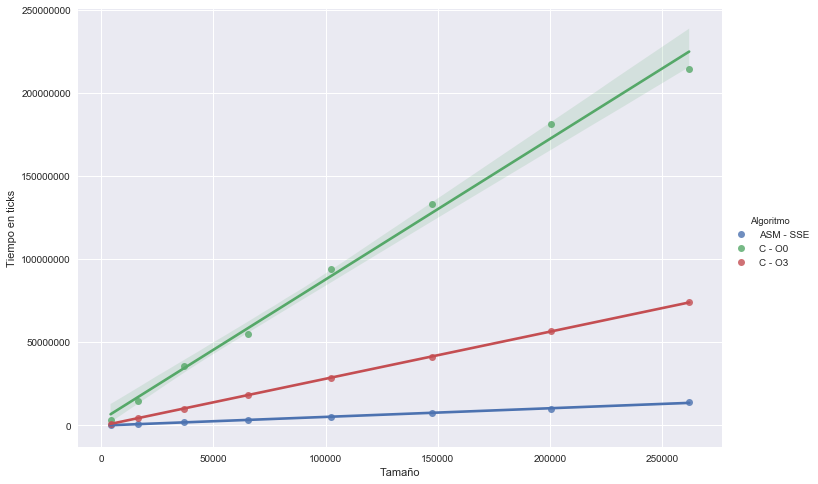
\includegraphics[scale=0.5]{img/maxCloser_CvsASMvsO3.png}
\end{center}

Podemos ver claramente como el filtro implementado en ASM corre más rápido que en C, de hecho, al incrementar el tamaño de la imagen la diferencia es aún más notable. Si bien hay una amplia mejora al compilar con optimizaciones O3, no llega a mejorar la versión de ASM. Esto es un comportamiento esperable ya que en C estamos yendo a buscar el pixel a memoria por cada pixel del kernel, en cambio en ASM con las instrucciones SIMD cada 7 pixeles lo pedimos 2 veces. Además, en ASM aprovechamos y hacemos las cuentas para el pixel destino en paralelo.

\subsection{Experimantación}
Queremos ver cómo impacta en ambas implementaciones si agrandamos el tamaño de kernel. Vamos a correr los mismos tests que antes, pero ahora en vez que del kernel sea 7x7 será de 11x11.

Nuestra hipótesis, es que esta medida va a afectar con más contundencia a la implementación de C, si bien en ASM va a tardar más, en relación al kernel mas chico, no le va afectar tanto. Esto es debido a que, en C trae cada pixel del kernel uno por vez, y como son casi 2.5 veces más, la cantidad de píxeles en el kerenel, esperamos una performance peor en este orden. Pero en ASM aprovechando la paralelización de datos, levantamos 11 píxeles con 3 llamadas a memoria nada más.

\begin{center} 
	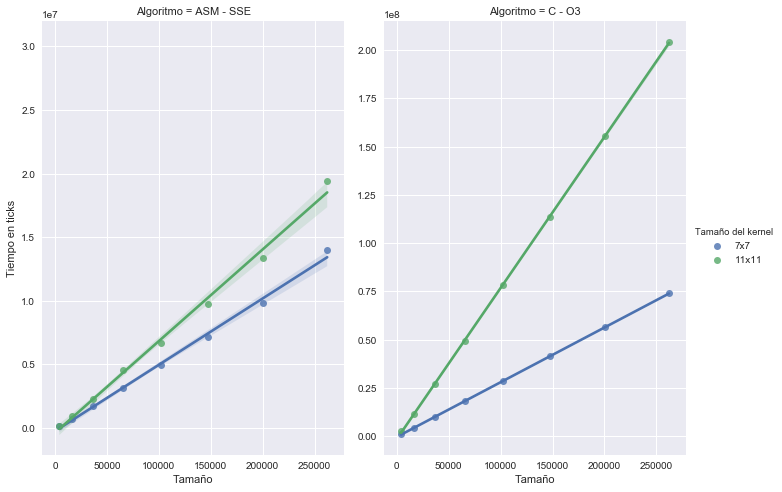
\includegraphics[scale=0.5]{img/maxCloser_KERNEL.png}
	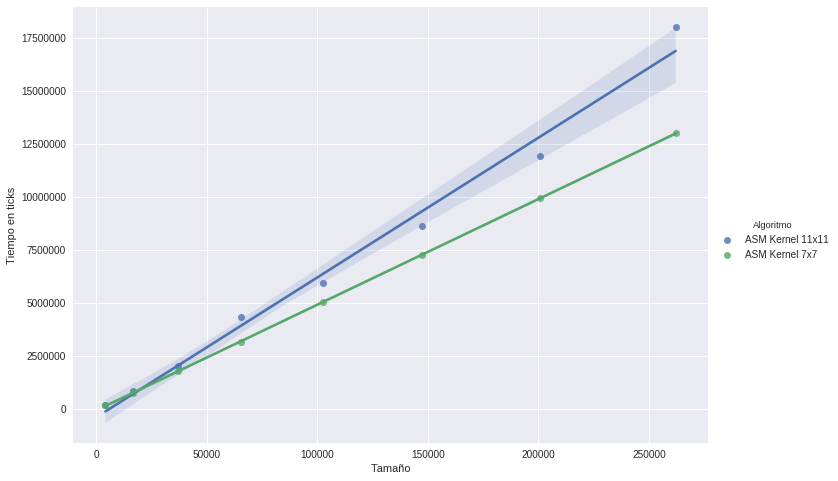
\includegraphics[scale=0.5]{img/maxCloser_KERNEL_ASM.png}
	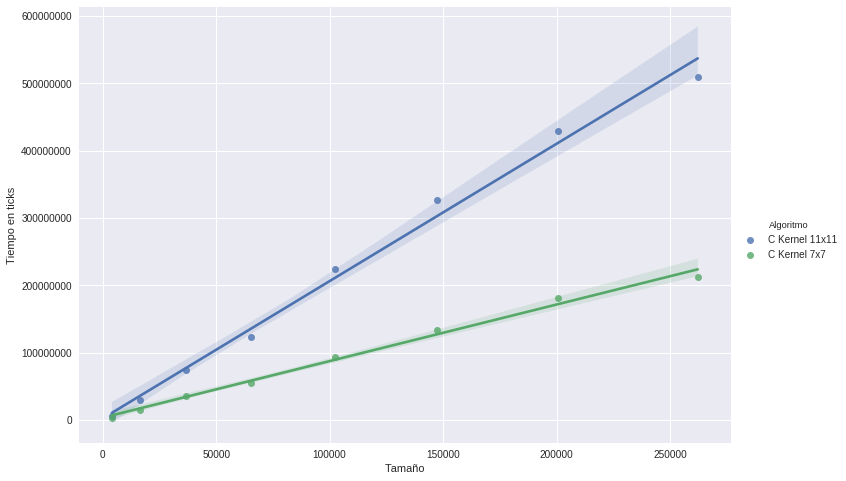
\includegraphics[scale=0.5]{img/maxCloser_KERNEL_C.png}
\end{center}

Si observamos los gráficos, podemos ver como en C con el kernel de 11x11 tarda casi 2,5 veces más, como la relación de diferencia de pixeles en los kernels, y para ASM hay nada mas una diferencia de 1,2 y 1,4 para instancias más grandes. Como habíamos predicho en la hipótesis, este cambio en el tamaño del kernel, afectó bastante más a la implementación de C que a la de ASM.

